% Copyright 2007 by Till Tantau
%
% This file may be distributed and/or modified
%
% 1. under the LaTeX Project Public License and/or
% 2. under the GNU Public License.
%
% See the file doc/licenses/LICENSE for more details.


\lecture[3]{Visualizing and Summarizing}{lecture-text}

\subtitle{means, medians, and plots}

\date{20 January 2015}


\begin{document}

\begin{frame}
  \maketitle
\end{frame}

% Overview of the problem:
%   different scales of data
% Measures of Center:
%   median
%   mean
%   comparison
% Boxplots:
%   quartiles
%   outliers
%   compared to histograms
% Visualizing relationships
%   categorical-categorical: stacked freqs
%   numeric-categorical: boxplots or dotplots
%   numeric-numeric: scatterplots



%%%%%
\begin{frame}{Overview}
    Goal: describe a dataset, i.e.
    \begin{enumerate}
        \item summarize important quantities (statistics)
        \item and visualize the data (plots)
    \end{enumerate}

    \vspace{3em}

    Like the histogram,
    these are \alert{descriptive statistics}.
\end{frame}


%%%%%
\begin{frame}\frametitle<presentation>{Outline}
  \tableofcontents
\end{frame}


%%%%% %%%%%
\section{Measures of Center: median and mean}


%%%%%
\begin{frame}{The Median}

    The \alert{median} of a collection of $n$ observations
    is:
    \begin{enumerate}
        \item (\textbf{$n$ odd}) the middle value.
        \item (\textbf{$n$ even}) the average of the middle two values.
    \end{enumerate}

    \vspace{3em}
    \pause

    \structure{Example:} Weight gain of lambs:
    \begin{center}
        \begin{tabular}{cccccc}
            11 & 13 & 19 & 2 & 10 & 1
        \end{tabular}
    \end{center}

    \pause

    \vspace{3em}

    \structure{``Example:''} Weight gain of baby sharks:
    \begin{center}
        \begin{tabular}{cccccc}
            11 & 13 & 190 & 2 & 10 & 1
        \end{tabular}
    \end{center}

\end{frame}


%%%%%
\begin{frame}{The Mean}

    The \alert{mean} (or ``average'') of a collection of observations is:
    \begin{enumerate}
        \item the sum of the observations, divided by the number of observations:
            \[
                \bar y = \frac{ y_1 + \cdots + y_n }{ n  }
            \]
    \end{enumerate}

    \pause

    \structure{Note:} the sum of deviations from the mean are always zero.
    \[
        (y_1 - \bar y) + (y_2 - \bar y) + \cdots + (y_n - \bar y) = 0
    \]

    \pause
    \vspace{2em}

    \structure{Example:} Weight gain of lambs:
    \begin{center}
        \begin{tabular}{cccccc}
            11 & 13 & 19 & 2 & 10 & 1
        \end{tabular}
    \end{center}

    \pause
    \vspace{2em}

    \structure{``Example:''} Weight gain of baby sharks:
    \begin{center}
        \begin{tabular}{cccccc}
            11 & 13 & 190 & 2 & 10 & 1
        \end{tabular}
    \end{center}

\end{frame}


%%%%%
\begin{frame}{Median vs Mean; Robustness}

    A statistic is \alert{robust} if it doesn't change much\\
    even if a small number of observations change by a lot. \\

    \vspace{3em}

    \structure{Think of:} ``robust to error''.

    \vspace{3em}

    \structure{Conversely,} robust statistics tend to ``not use all the data''.

    \vspace{3em}
    \pause

    The median is robust, the mean is not.

    \vspace{2em}

    \textbf{Think of a situation} when the median be a better choice than the mean.

    And, vice-versa.

\end{frame}


%%%%%
\begin{frame}{the Quartiles}

    \textbf{Quartiles} divide the data into \emph{quarters}:
    \begin{itemize}
        \item the \alert{first quartile} is the median of the {lower half}
        \item (the \alert{second quartile} is the median)
        \item the \alert{third quartile} is the median of the {upper half}
    \end{itemize}

    \vspace{2em}

    The \alert{interquartile range} (``\textbf{IQR}'') is the difference between the third and the first quartiles.

    \pause
    \vspace{2em}

    \structure{Example:} blood pressures.
    \begin{center}
        \begin{tabular}{ccccccc}
            151 & 124 & 132 & 170 & 146 & 124 & 113
        \end{tabular}
    \end{center}

    \pause
    \vspace{2em}

    \structure{Example:} pulses.
    \begin{center}
        \begin{tabular}{cccccccccccc}
            62 & 64 & 68 & 70 & 70 & 74 & 74 & 76 & 76 & 78 & 78 & 80 
        \end{tabular}
    \end{center}

\end{frame}


\section{Boxplots}

%%%%%
\begin{frame}{Boxplots: the ``five-number'' summary}

    \begin{center}
        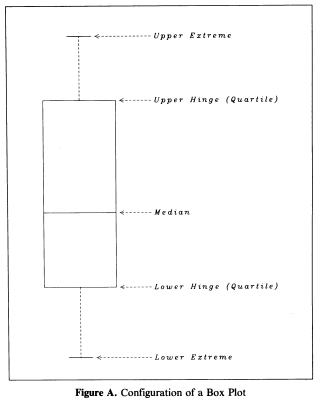
\includegraphics[height=.85\textheight]{boxplot-taxonomy.png}
        \figcaption{McGill, Tukey, \& Larson 1978}
    \end{center}

\end{frame}


%%%%%
\begin{frame}{Boxplots: modified}

    Medians and quartiles are \textbf{robust},
    but the maximum and minimum are \alert{not}.

    \vspace{2em}

    We'd like the boxplot to be robust. 

    \vspace{2em}

    \structure{Solution:}
    Extend the whiskers out only to the ``fences'':
    \[
        \text{( quartile )} \; \pm \; 1.5 \times \text{( IQR )} 
    \]

    \centering
    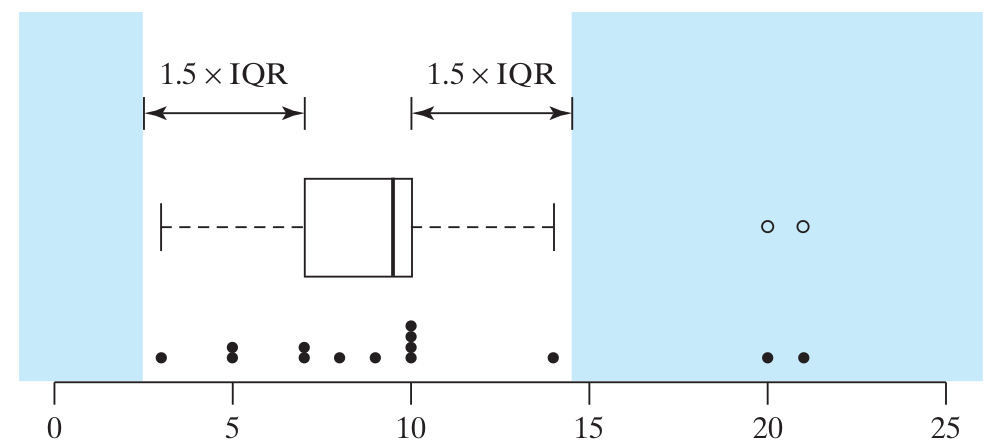
\includegraphics[width=0.8\textwidth]{modified-boxplot-fig_2_4_2.png}

\end{frame}

%%%%%
\begin{frame}{Comparison of the methods:}

  166 SoCal earthquakes magnitude ${}>3$ in 2014 \\
  {\small (from \url{http://service.scedc.caltech.edu/}) }

    \begin{center}
        \includegraphics<1>[width=\textwidth]{quakes-dotplot}
        \includegraphics<2>[width=\textwidth]{quakes-hist}
        \includegraphics<3>[width=\textwidth]{quakes-boxplot}
        \includegraphics<4>[width=\textwidth]{quakes-modified-boxplot}
    \end{center}

\end{frame}


%%%%% %%%%%
\section{Visualizing relationships}

\begin{frame}{More than one variable: relationships}

  Histograms, medians, means, and boxplots \\
  are all summaries of a \alert{single group} of numbers:\\
  \textbf{measurements} of a single variable.

  \vspace{2em}

  \structure{Often,} we measure \alert{more than one variable},
  and what we can do depends on the type of variables, e.g.
  \begin{itemize}
    \item \structure{categorical-categorical}: treatment $\times$ result \\ 
      -- how many fall in each combination of categories?
    \item \structure{categorical-numeric}: treatment $\times$ measurement \\ 
      -- how do the distributions of measurements in different categories compare?
    \item \structure{numeric-numeric}: measurement $\times$ measurement \\ 
      -- how do the two variables relate to each other?
  \end{itemize}

\end{frame}

\subsection{Stacked frequency plots}

%%%%%
\begin{frame}{Absolute frequencies, stacked}
    \begin{center}
        % \begin{column}{0.5\textwidth}
            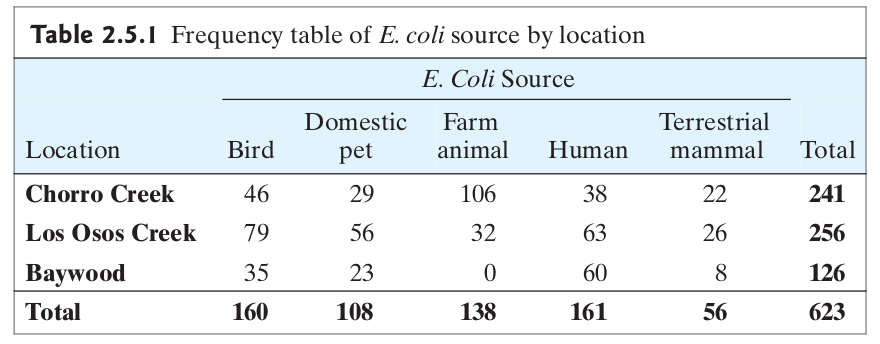
\includegraphics[width=.8\textwidth]{ecoli-counts-tab2_5_1.png}
        % \end{column}

        % \begin{column}{0.5\textwidth}
            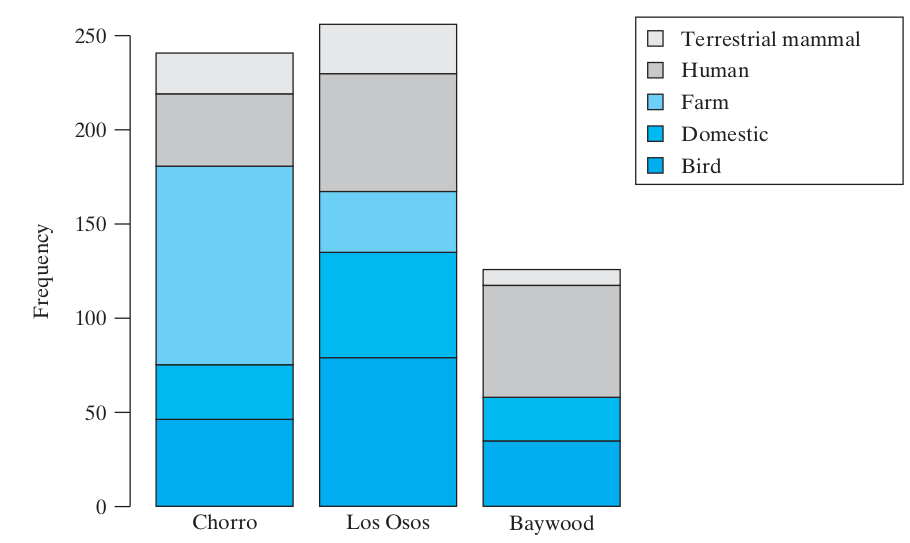
\includegraphics[width=.8\textwidth]{ecoli-counts-fig2_5_1.png}
        % \end{column}
    \end{center}
\end{frame}

%%%%%
\begin{frame}{Relative frequencies, stacked}
    \begin{center}
        % \begin{column}{0.5\textwidth}
            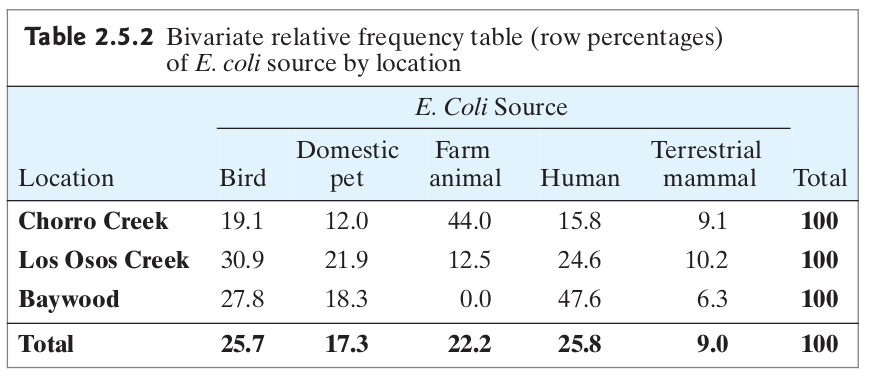
\includegraphics[width=0.8\textwidth]{ecoli-freqs-tab2_5_2.png}
        % \end{column}

        % \begin{column}{0.5\textwidth}
            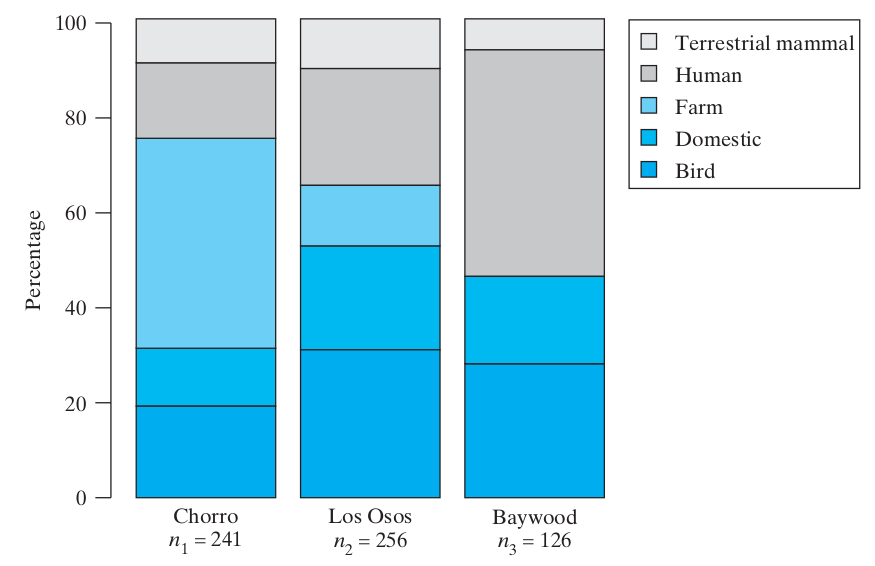
\includegraphics[width=0.8\textwidth]{ecoli-freqs-fig2_5_2.png}
        % \end{column}
    \end{center}
\end{frame}


%%%%%
\begin{frame}{What's the difference?}

  What does each one show more clearly than the other?

    \begin{columns}
        \begin{column}{0.5\textwidth}
    \begin{center}
            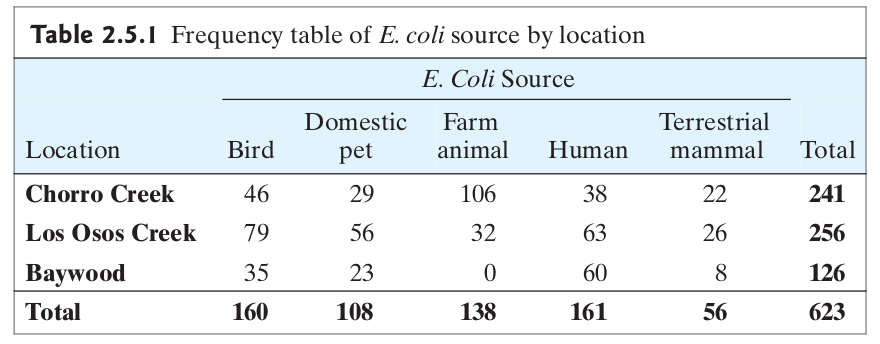
\includegraphics[width=.9\textwidth]{ecoli-counts-tab2_5_1.png}

            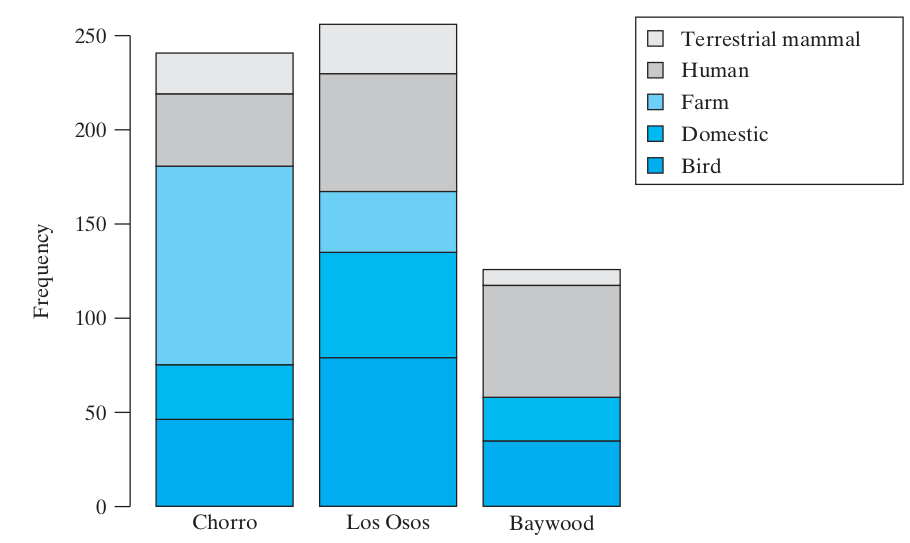
\includegraphics[width=.9\textwidth]{ecoli-counts-fig2_5_1.png}
    \end{center}
        \end{column}

        \begin{column}{0.5\textwidth}

    \begin{center}
            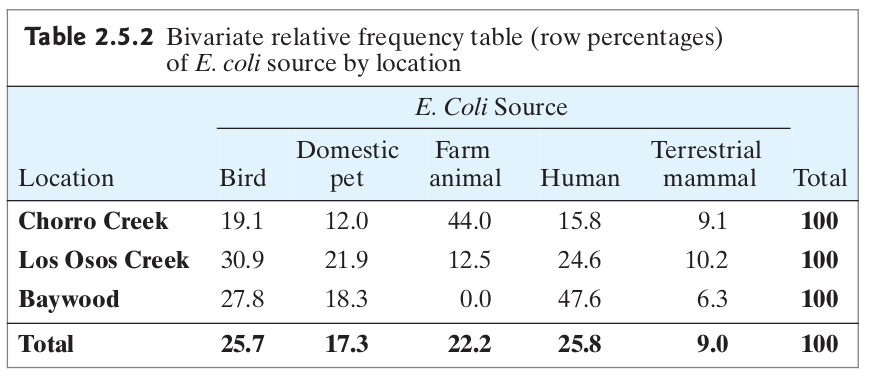
\includegraphics[width=.9\textwidth]{ecoli-freqs-tab2_5_2.png}

            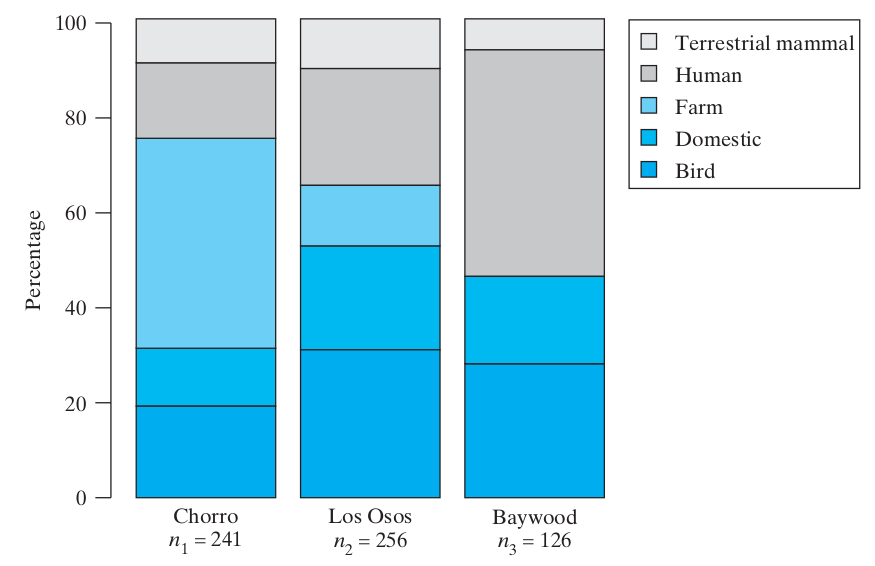
\includegraphics[width=.9\textwidth]{ecoli-freqs-fig2_5_2.png}
    \end{center}
\end{column}
\end{columns}

\end{frame}


%%%%% %%%%%
\subsection{Boxplots and dotcharts, by category}

%%%%%
\begin{frame}{Categorical--numeric}

    Earthquakes, again:
    \begin{center}
        \includegraphics<1>[width=\textwidth]{quakes-category-dotplot}
        \includegraphics<2>[width=\textwidth]{quakes-category-boxplot}
    \end{center}

\end{frame}


%%%%% %%%%%
\subsection{Scatter plots}

%%%%%
\begin{frame}{Numeric--numeric: Bivariate scatter plots}

  Earthquakes, again:
  \begin{center}
    \includegraphics<1>{quakes-mag-depth}
    \includegraphics<2>{quakes-mag-depth-lines}
    \includegraphics<3>{quakes-mag-time}
    \includegraphics<4>{quakes-mag-time-lines}
  \end{center}


\end{frame}


\section<article>{Summary}
\section<presentation>*{Summary}

\begin{frame}{Summary}
  \begin{enumerate}
    \item The median and mean are two summaries of \emph{location}.
    \item The median is more \emph{robust} to outliers,
    \item the mean is a better predictor of \emph{sums}.
    \item \emph{Quartiles} divide the data into quarters,
    \item and can be depicted in \emph{boxplots}.
    \item Relationships between variables can be depicted with
    \begin{itemize}
      \item stacked frequencies
      \item parallel boxplots
      \item scatterplots
    \end{itemize}
  \end{enumerate}
  \vspace{2em}

  \structure{Rule of thumb:}
  maximize information while minimizing ink.
\end{frame}

% homework
\begin{frame}{Homework}
  \begin{center}

  2.3.15, 2.3.16

  \vspace{2em}


  2.4.3
  
  \vspace{2em}

  2.5.2

  \end{center}
\end{frame}


\end{document}
